\subsection{RisingWave}

RisingWave merupakan \textit{cloud-native streaming database}. Setelah menghubungkan sumber \textit{stream}, pengguna dapat membuat kueri analisis dengan mendefinisikan \textit{materialized view}, yang diperbarui secara inkremental pada RisingWave \textit{streaming engine} \parencite{risingwave}.

Berikut adalah keuntungan RisingWave:

\begin{enumerate}
    \item Mudah dipelajari karena merupakan ekstensi dari sintaks PostgreSQL.
    \item Mudah dioperasikan dan memiliki kebutuhan sumber daya yang lebih rendah karena ditulis dalam bahasa sistem Rust.
    \item Mendukung berbagai sumber data dan mampu mengirimkan (\textit{sink}) data ke dalam berbagai sumber, seperti mengambil data dari Apache Kafka lalu hasilnya dikirim ke ClickHouse. RisingWave mendukung integrasi dengan PostgreSQL CDC dan Apache Kafka sebagai sumber (\textit{source}) dan tujuan data (\textit{sink}).
    \item Menjamin konsistensi pada \textit{materialized view} dengan menggunakan \textit{snapshot}.
\end{enumerate}

\begin{figure}[htbp]
    \centering
    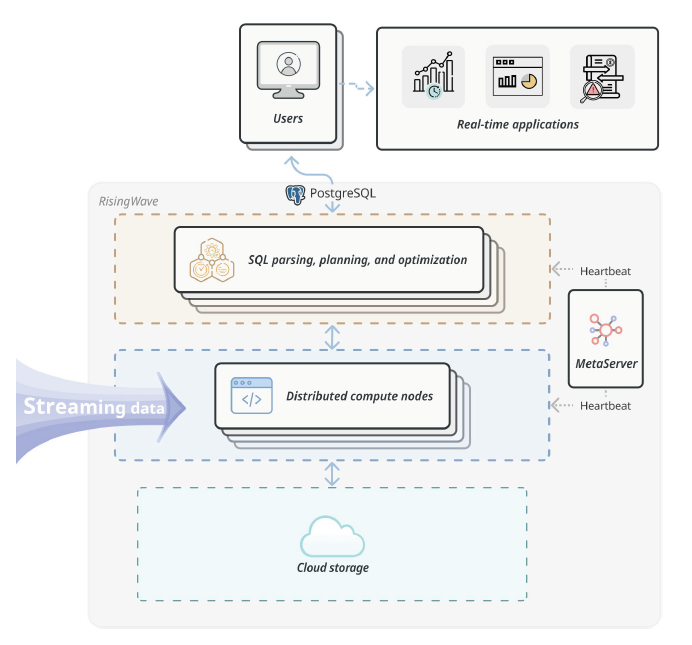
\includegraphics[width=0.8\textwidth]{resources/chapter-2/risingwave.png}
    \caption{Arsitektur RisingWave \parencite{risingwave}}
    \label{fig:risingwave-architecture}
\end{figure}

Node komputasi pada RisingWave terdiri atas \textit{batch engine} dan \textit{streaming engine}. \textit{Batch engine} meliputi \textit{query execution engine} dan \textit{exchange service} untuk menukar data antar node komputasi. \textit{Streaming engine} dibangun atas model aktor pada pemrograman konkuren. Mesin ini berinteraksi langsung dengan \textit{frontend} dan melayani \textit{stream data}. Selain itu, terdapat \textit{meta service} yang berperan sebagai layanan sentral untuk menyimpan metadata seperti keadaan kluster, katalog sistem, keanggotaan kluster, dan lain-lain \parencite{risingwave}.